\documentclass[11pt,a4paper]{article}
\usepackage[T1]{fontenc}\usepackage[utf8]{inputenc}\usepackage[spanish,es-nodecimaldot]{babel}
\usepackage{lmodern,geometry,booktabs,graphicx,hyperref}
\geometry{margin=2cm}\setlength{\parindent}{0pt}\setlength{\parskip}{6pt}\setlength{\emergencystretch}{3em}
\begin{document}
\begin{center}{\LARGE ATM: investigación y decisión NO-GO}\par
Cristian Acevedo, Guillermo Arriaza y Eduardo Ponce\par 25 de noviembre de 2026\end{center}
\textbf{No sustituir el BIN activo.} Se evaluaron 191 configuraciones; la selección
usó solo ocho prefijos de 12000 ticks. No se reajustó tras ver el test.
El modelo tiene tres regímenes, momentum corto/largo, confirmación, exposición,
reserva y stops de volatilidad. La elegida usa 16/64 ticks, revisión 8, dos
confirmaciones, entrada +4, salida -4 y stop entre 12 y 40 puntos. La grilla
también incluye medias, persistencia, ruptura, pendiente y exposiciones de 25 a 100\%.

\begin{center}\small\begin{tabular}{lrrrrr}\toprule
Política & Media & Ventajas/8 & Peor final & DD máx.\% & Comisión media\\\midrule
No\_operar & 10.000 & 6 & 10.000 & 0,00 & 0 \\
Mantener\_teorico & 9.679 & 0 & 8.315 & 60,73 & 5 \\
Mantener\_SPI & 9.687 & 2 & 8.315 & 60,73 & 9 \\
Momentum32 & 12.725 & 6 & 8.615 & 61,11 & 271 \\
Tendencia\_lenta & 10.971 & 5 & 8.540 & 50,55 & 119 \\
SMA10 & 5.467 & 0 & 4.577 & 54,47 & 4.833 \\
Agresiva & 9.558 & 4 & 4.531 & 63,86 & 76 \\
Candidata\_anterior & 10.234 & 6 & 8.284 & 30,34 & 106 \\
ATM & 11.814 & 5 & 7.717 & 49,38 & 412 \\
\bottomrule\end{tabular}\end{center}
\begin{center}\resizebox{\linewidth}{!}{\begin{tabular}{lrrrrrrrr}\toprule
Serie & Momentum32 & ATM & Mantener & Ventaja ATM & Compras & Ventas & Comisión & DD\%\\\midrule
AMD enero & 19.312 & 13.356 & 8.315 & 5.041 & 65 & 63 & 640 & 30,56 \\
AMD mayo & 11.490 & 9.227 & 9.647 & -420 & 34 & 34 & 340 & 36,04 \\
Apple 2022 & 12.528 & 12.740 & 11.063 & 1.677 & 46 & 46 & 460 & 31,65 \\
Apple 2023 & 13.555 & 10.175 & 10.371 & -196 & 46 & 46 & 460 & 36,85 \\
Meta 2022 & 13.700 & 16.366 & 9.695 & 6.671 & 37 & 37 & 370 & 17,46 \\
Netflix 2022 & 8.615 & 10.816 & 9.179 & 1.637 & 42 & 42 & 420 & 36,46 \\
Netflix 2023 & 8.929 & 7.717 & 9.170 & -1.453 & 31 & 30 & 305 & 49,38 \\
Tesla 2022 & 13.671 & 14.115 & 9.995 & 4.120 & 30 & 30 & 300 & 29,34 \\
\bottomrule\end{tabular}}\end{center}

ATM gana en 5/8, frente a 6/8. La mediana relativa baja de 24,90\% a 16,50\%;
la peor ventaja pasa de -6,14\% a -15,85\%. El drawdown mejora de 61,11\% a
49,38\%, pero la comisión media sube de 270,63 a 411,88. Ninguna variante
elegible cumplió simultáneamente las seis puertas descriptivas de serie completa.
Esto no autoriza seleccionar retrospectivamente otra configuración por el test.

\textbf{Validación temporal.} LOCO: 6/8 frente a 5/8 histórico; LOSO: 5/8 frente
a 6/8; walk-forward: 14/24 frente a 14/24. Cada selección usa su entrenamiento,
sin su empresa/serie excluida o ventana futura. Son datos conocidos de desarrollo,
no una validación independiente en series secretas. WF reinicia la cartera y
los indicadores en cada ventana. Se reprodujeron las selecciones de referencia.

\begin{center}\small\begin{tabular}{lrrrr}\toprule
Política & Ternas +/56 & Peor suma & Peor ventaja & Ventaja media\\\midrule
Momentum32 & 56 & 29.034 & 660 & 9.137 \\
ATM & 52 & 27.119 & -2.069 & 6.404 \\
Tendencia\_lenta & 52 & 27.154 & -2.859 & 3.875 \\
SMA10 & 0 & 14.543 & -14.848 & -12.638 \\
Mantener\_SPI & 31 & 26.688 & -90 & 22 \\
No\_operar & 44 & 30.000 & -1.429 & 962 \\
Mantener\_teorico & 0 & 26.664 & 0 & 0 \\
\bottomrule\end{tabular}\end{center}
Se evaluaron las 56 ternas distintas y, adicionalmente, 120 con repetición por
política. Se suman patrimonios de rondas independientes de 10000 iniciales.
No son resultados de la competencia oficial ni determinan una calificación.

\textbf{Contabilidad.} La orden se ejecuta al precio siguiente, máximo 63,
comisión 5 por fill positivo y sin deuda ni corto. Se cotejaron 160000 ticks de
decisiones y cartera con una implementación independiente; cero discrepancias.
El CSV completo está comprimido sin pérdida. Se conservaron las configuraciones
perdedoras, compras, ventas, exposición y nueve estreses sintéticos.

\textbf{Hardware: fase no habilitada.} Por NO-GO no se tradujo ATM a RV32E,
no se ejecutó RTL ATM ni el banco oficial con ATM, y no se sintetizó ni generó
un BIN nuevo. No se atribuyen a ATM ciclos, CPI o recursos de otra política.
La referencia activa sigue en 1260 LC, 9 BRAM, Fmax 50,19 MHz y 321 ciclos
máximos observados a 12,5 MHz (25,68 us). Sus pruebas Icarus se repitieron sin
modificar los archivos protegidos. No se programó físicamente la FPGA.

\textbf{Reproducción:}\par
\path{python -X utf8 -B proyecto4/alternativas/atm_adaptativa/ejecutar_todo.py}\par
Las reglas, el ranking y las puertas están en PROTOCOLO.json. El informe completo
en Markdown detalla las limitaciones; los CSV y firmas permiten revisar cada
resultado. La decisión corresponde a esta grilla, no a una imposibilidad general
de superar al baseline.

\clearpage\section*{Patrimonios: ATM, Momentum32 y mantener}
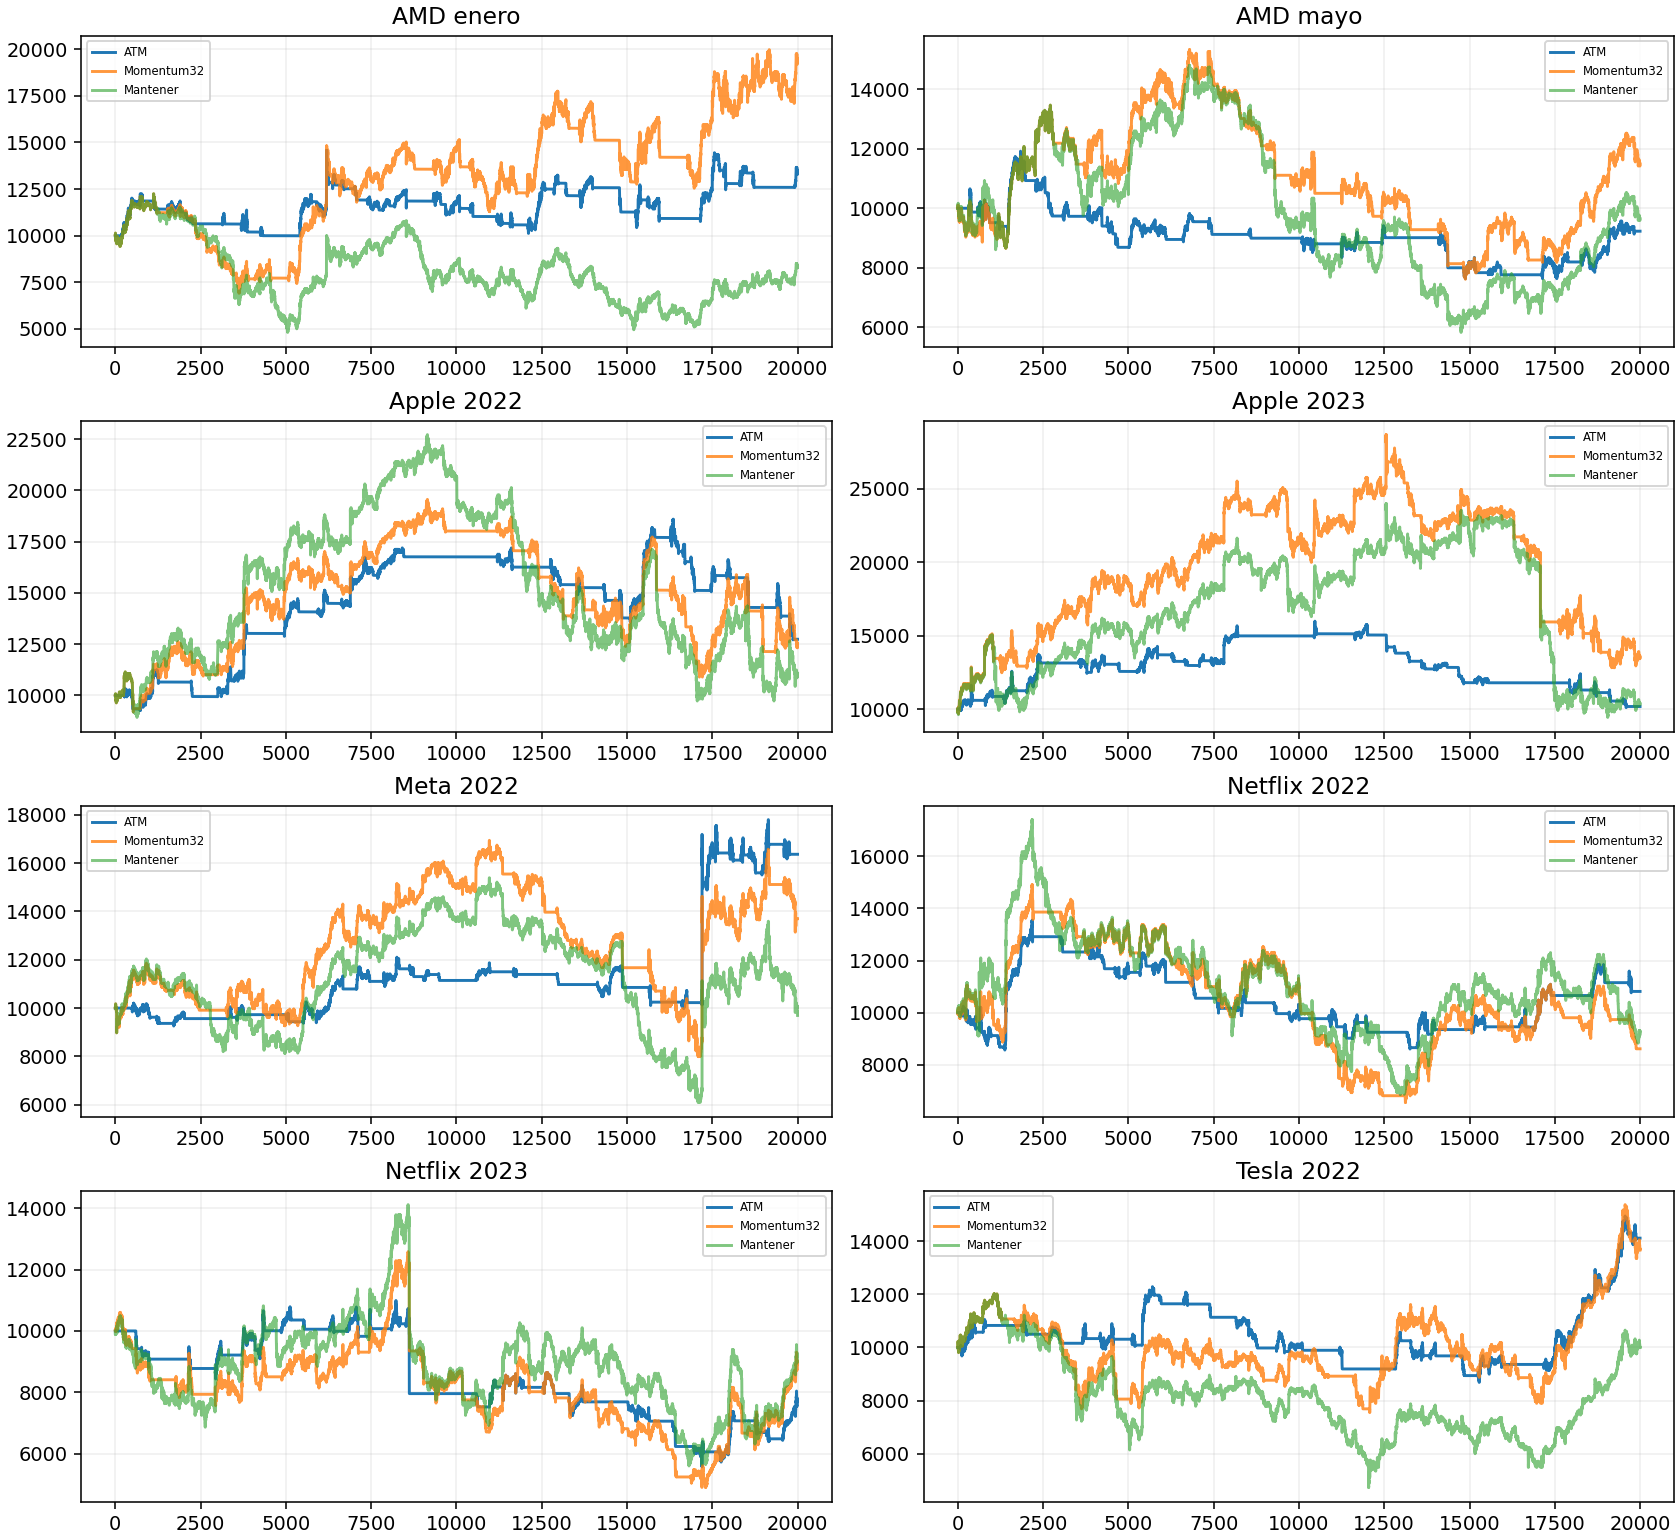
\includegraphics[width=\linewidth,height=.87\textheight,keepaspectratio]{resultados/patrimonios.png}
\clearpage\section*{Drawdown: comparación por serie}
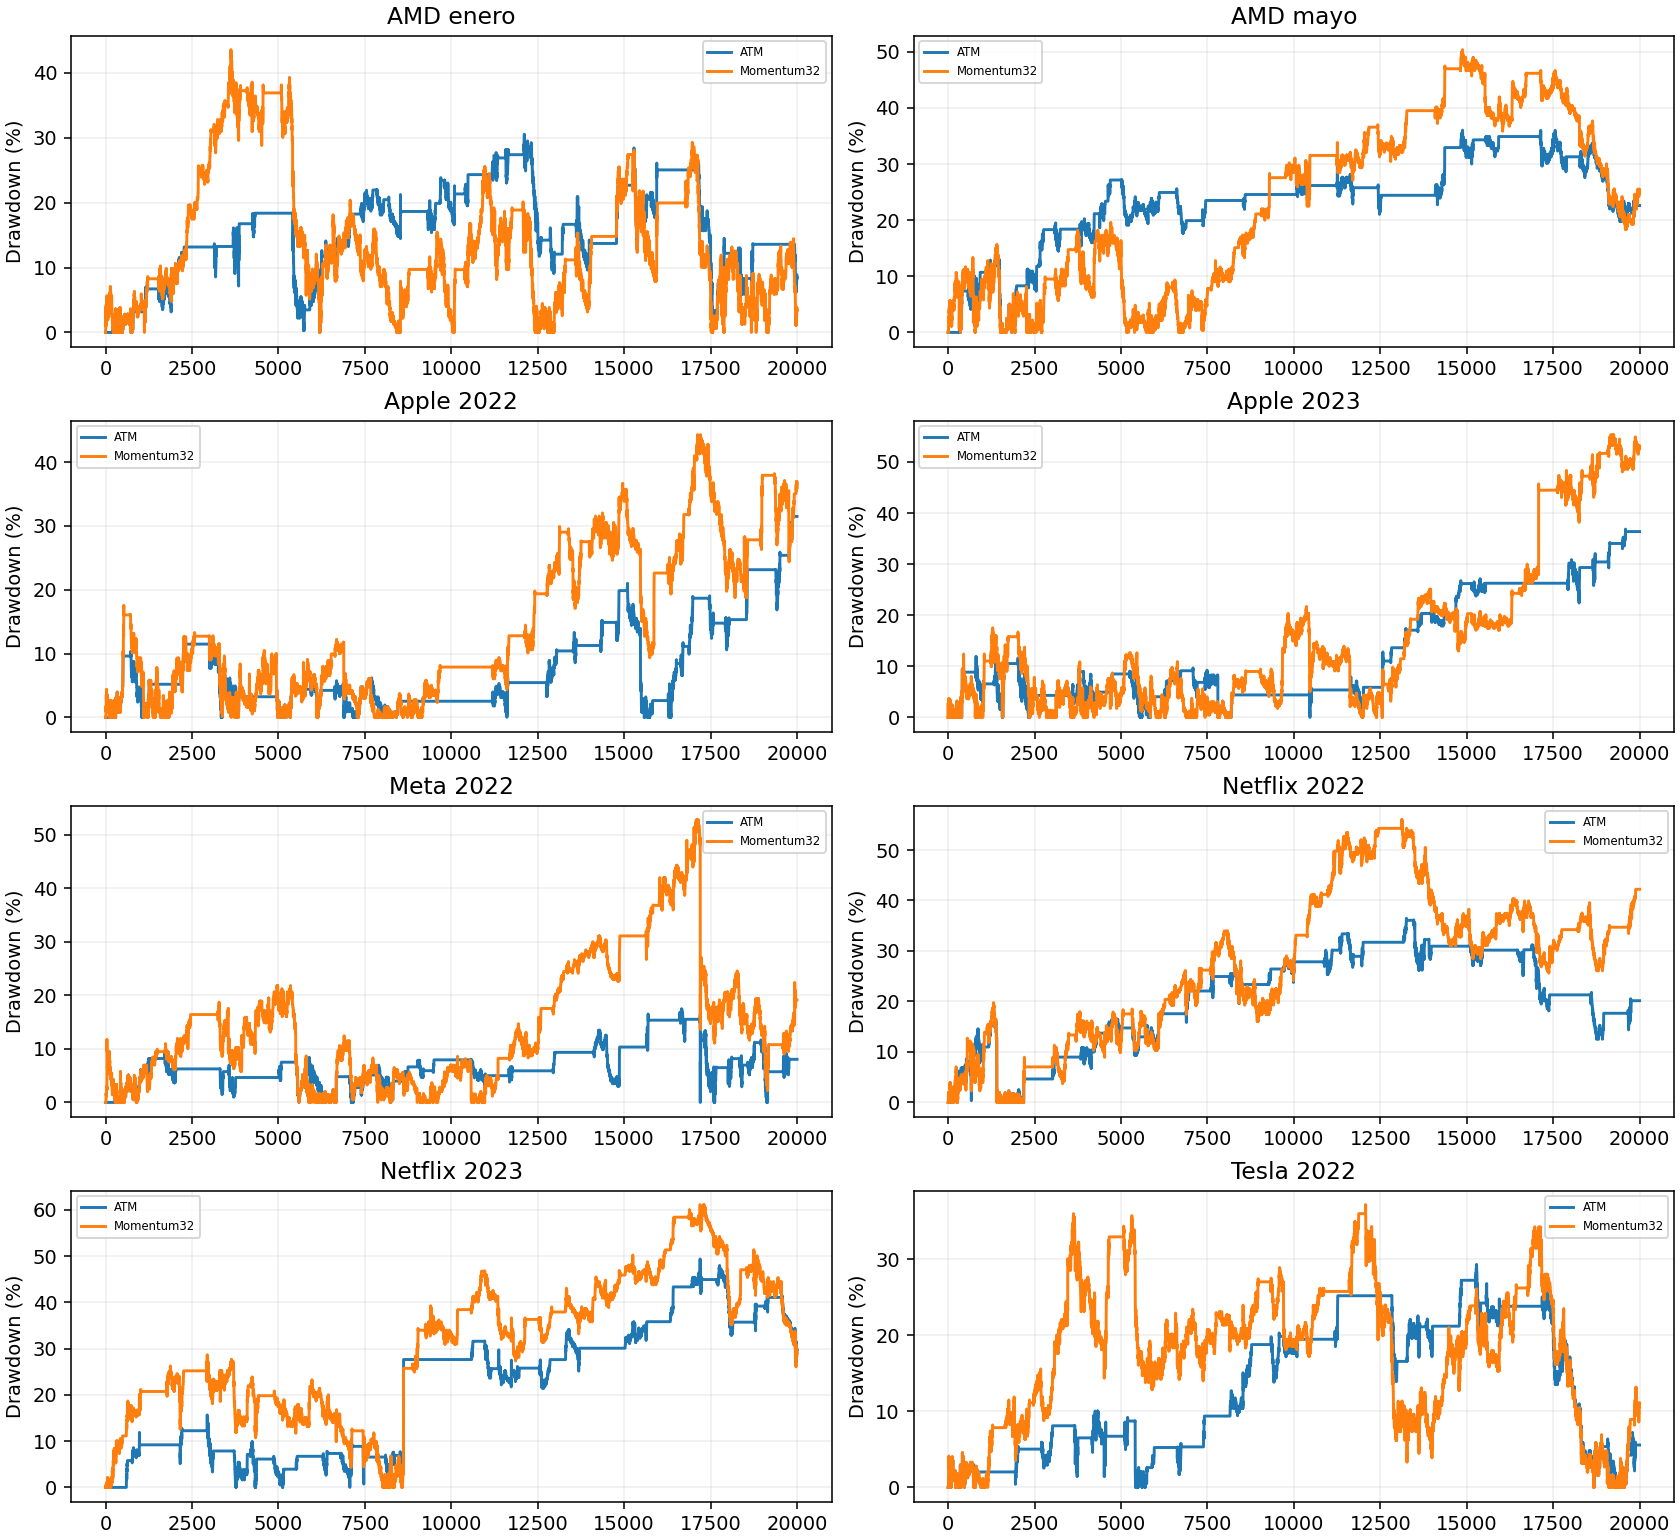
\includegraphics[width=\linewidth,height=.87\textheight,keepaspectratio]{resultados/drawdowns.png}
\clearpage\section*{Compras y ventas ATM al precio de ejecución}
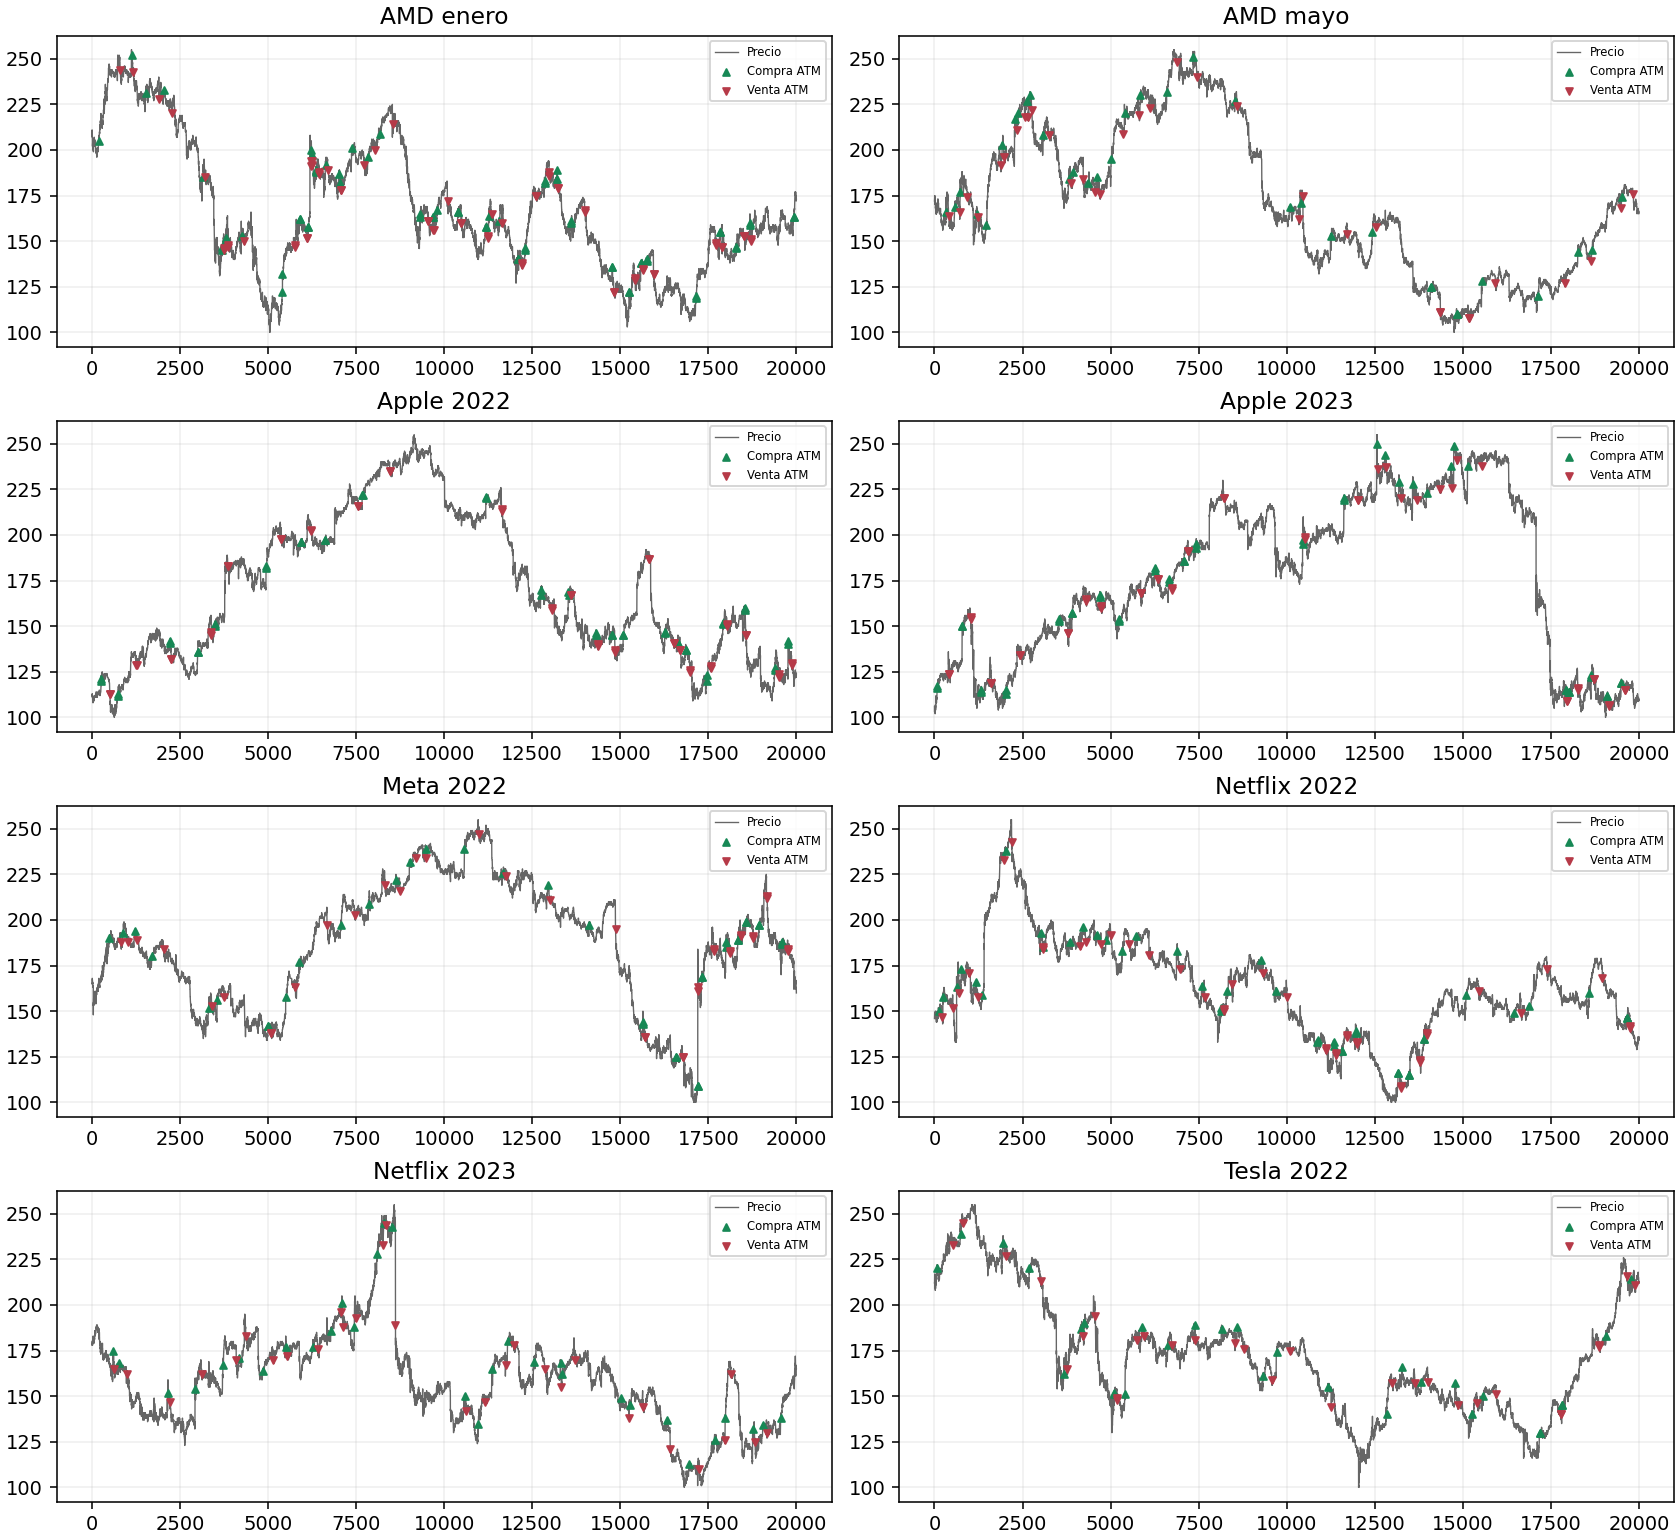
\includegraphics[width=\linewidth,height=.87\textheight,keepaspectratio]{resultados/compras_ventas.png}
\end{document}
